\documentclass[10pt,a4paper,english]{article}
\usepackage{babel}
\usepackage{ae}
\usepackage{aeguill}
\usepackage{shortvrb}
\usepackage[latin1]{inputenc}
\usepackage{tabularx}
\usepackage{longtable}
\setlength{\extrarowheight}{2pt}
\usepackage{multicol}
\usepackage{amsmath}
\usepackage{graphicx}
\usepackage{color}
\usepackage{multirow}
\usepackage{float}\usepackage{ifthen}
\usepackage{titletoc}
\usepackage{lipsum}
\usepackage{fancyhdr}
\usepackage[DIV12]{typearea}
% generated by Docutils <http://docutils.sourceforge.net/>
\newlength{\admonitionwidth}
\setlength{\admonitionwidth}{0.9\textwidth}
\newlength{\docinfowidth}
\setlength{\docinfowidth}{0.9\textwidth}
\newlength{\locallinewidth}
\newcommand{\optionlistlabel}[1]{\bf #1 \hfill}
\newenvironment{optionlist}[1]
{\begin{list}{}
  {\setlength{\labelwidth}{#1}
   \setlength{\rightmargin}{1cm}
   \setlength{\leftmargin}{\rightmargin}
   \addtolength{\leftmargin}{\labelwidth}
   \addtolength{\leftmargin}{\labelsep}
   \renewcommand{\makelabel}{\optionlistlabel}}
}{\end{list}}
\newlength{\lineblockindentation}
\setlength{\lineblockindentation}{2.5em}
\newenvironment{lineblock}[1]
{\begin{list}{}
  {\setlength{\partopsep}{\parskip}
   \addtolength{\partopsep}{\baselineskip}
   \topsep0pt\itemsep0.15\baselineskip\parsep0pt
   \leftmargin#1}
 \raggedright}
{\end{list}}
% begin: floats for footnotes tweaking.
\setlength{\floatsep}{0.5em}
\setlength{\textfloatsep}{\fill}
\addtolength{\textfloatsep}{3em}
\renewcommand{\textfraction}{0.5}
\renewcommand{\topfraction}{0.5}
\renewcommand{\bottomfraction}{0.5}
\setcounter{totalnumber}{50}
\setcounter{topnumber}{50}
\setcounter{bottomnumber}{50}
% end floats for footnotes
% some commands, that could be overwritten in the style file.
\newcommand{\rubric}[1]{\subsection*{~\hfill {\it #1} \hfill ~}}
\newcommand{\titlereference}[1]{\textsl{#1}}
% end of "some commands"
\ifthenelse{\isundefined{\hypersetup}}{
\usepackage[colorlinks=true,linkcolor=blue,urlcolor=blue]{hyperref}
}{}
\title{PBK}
\author{}
\date{}
\hypersetup{
pdftitle=TexBooks,
pdfauthor={INSERT AUTHOR}
}
\raggedbottom
\lhead{Example Template by Matt}
\begin{document}
\maketitle
%___________________________________________________________________________
\begin{center}
\begin{tabularx}{\docinfowidth}{lX}
\textbf{Author}: &
	Eugene A. Fedotov, Matthew Douglass, Jovaughn Chin \\
\textbf{Version}: &
	0.1 \\
\textbf{Licence}: &
	\textsc{gnu} Free
	Documentation License \\
\end{tabularx}
\end{center}

\setlength{\locallinewidth}{\linewidth}


The PBK package aims to be a Portable Kit for open-source Books. It is meant to provide a diverse selection of common graphical diagrams in select subjects. Currently, the focus is on compilers and programming in Java.


%___________________________________________________________________________

\pdfbookmark[0]{Dependencies}{dependencies}
\section*{Dependencies}
\label{dependencies}

The following libraries are required to run PBK:
\begin{itemize}
\item {} 
\href{https://www.ctan.org/pkg/pgf}{PGF} 3.0
\end{itemize}


%___________________________________________________________________________

\pdfbookmark[1]{Libraries}{libraries}
\section*{Libraries}
\label{libraries}



%___________________________________________________________________________

\section*{Agenda \small{(subject to change)}}
\subsection{Sprint 1 : 3/9 - 3/13}
\begin{enumerate}
\item Decide on a set of diagrams for each person.
\item Pick one diagram. Create a hard (specific with no customization) example that illustrates the exact look.
\end{enumerate}
\subsection{Sprint 2 : 3/16 - 3/20}
\begin{enumerate}
\item Consider what possible options can be implemented.
\item Refactor the code to implement those options.
\end{enumerate}
\subsection{Sprint 3 : 3/23 - 3/27}
\begin{enumerate}
\item Check for issues. Scalability? Color? 
\item Add the function to the package.
\item Update doc.
\end{enumerate}
\subsection{Sprint 3 : 3/30 - 4/3}
\begin{enumerate}
\item Work on the next diagram.
\end{enumerate}
\subsection{Sprint 4 : 4/6 - 4/9}
\begin{enumerate}
\item TBD
\end{enumerate}
%___________________________________________________________________________



\newpage
\thispagestyle{fancy}
%%matts stuff
\begin{flushleft}

%%If I just want to link the images instead of the code
%%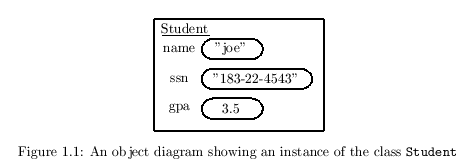
\includegraphics{class1.PNG}
\subsection*{Arrays}

\subsection*{Expressions}

\subsection*{Classes}

\subsection*{Objects}

\subsection*{State Machines}

\section{User Input}
Users will be able to create diagrams by editing a section near the top of the latex code.  This section will be clearly defined, easily editedable and understandable.  Below is a work in progress of some latex code that the user will have to edit to create a diagram that fits their specs. The example below is specifically used when making array diagrams and is far from final.

\begin{quote}{\ttfamily \raggedright \noindent
User Input Below~\\
{\textbackslash}newcommand{\{}{\textbackslash}ArrayName{\}}~\\
{\{}ARRAY NAME HERE{\}}~\\
{\textbackslash}newcommand{\{}{\textbackslash}Caption{\}}~\\
{\{}CAPTION HERE{\}}~\\
{\textbackslash}newcommand{\{}{\textbackslash}ArrayLengthMinusOne{\}}~\\
{\{}ARRAY LENGTH HERE{\}}~\\
{\textbackslash}newcommand{\{}{\textbackslash}0{\}}~\\
{\{}PLACE 0 VALUE HERE{\}}~\\
{\textbackslash}newcommand{\{}{\textbackslash}1{\}}~\\
{\{}PLACE 1 VALUE HERE{\}}~\\
{\textbackslash}newcommand{\{}{\textbackslash}2{\}}~\\
{\{}PLACE 2 VALUE HERE{\}}~\\
{\textbackslash}newcommand{\{}{\textbackslash}3{\}}~\\
{\{}PLACE 3 VALUE HERE{\}}~\\
{\textbackslash}newcommand{\{}{\textbackslash}4{\}}~\\
{\{}PLACE 4 VALUE HERE{\}}~\\
User Input Above~\\
}\end{quote}

The user will find the location in the template that clearly states "User Input Below" and edit below that until they come to "User Input Above".  The user will edit only the statements that are in CAPS being careful not to edit anything besides that.  For example if the user wanted to create an array diagram that holds 4 values they would look for "ARRAY LENGTH HERE".  After finding this they would replace the text in CAPS with an integer.  The user would then compile the LATEX code to find a array diagram to the users specs.  Above the user input area there will be information regarding what inputs are acceptable for the template. 


\end{flushleft}

\pdfbookmark[1]{Change History}{change}
\newpage
\begin{multicols}{2} % Two-column layout throughout the main article text

\section*{Change History}
v0.1\\
\indent General: Initial version \dotfill 1
\end{multicols}

\end{document}
